\chapter{Neural Network Model Training and Inference}
\label{Model::Training}

\begin{figure}[!ht]
    \centering
    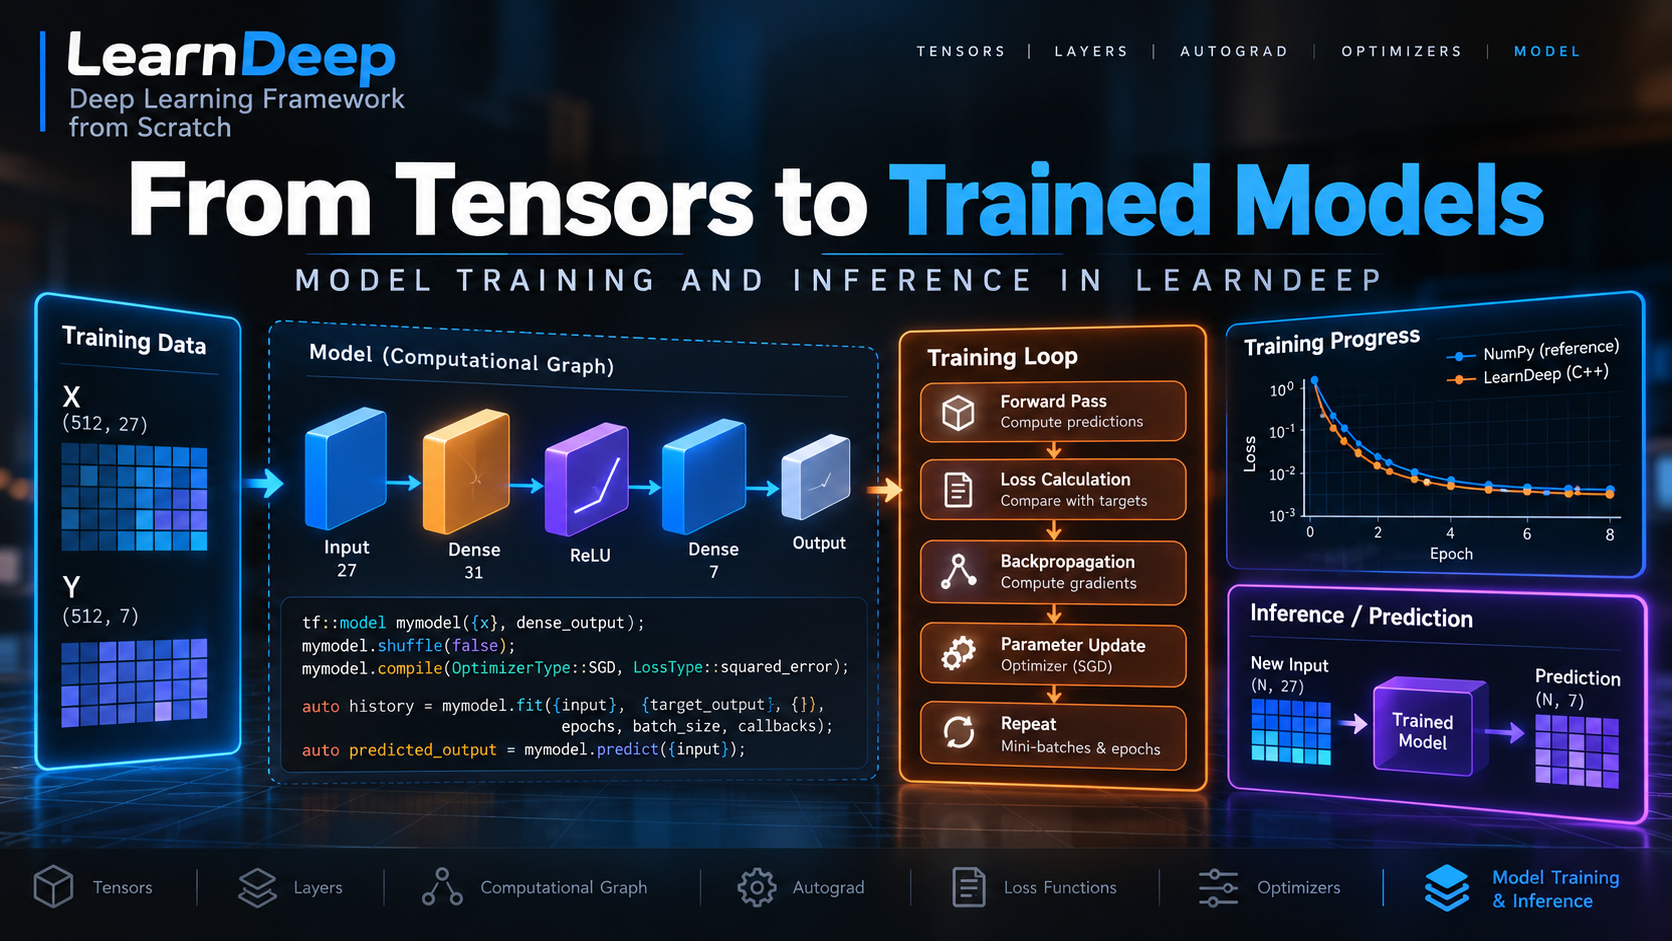
\includegraphics[width=\textwidth]{../../images/09_LearnDeep_ From Tensors to Trained Models.png
    }
\end{figure}

\paragraph{}
So far, we have developed the fundamental components required
to construct and train a neural network, including tensors,
layers, loss functions, optimizers, and automatic differentiation.

The next step is to bring these components together into a
complete training and inference workflow.

In this chapter, we will explore the public model API exposed
by LearnDeep and understand how it orchestrates the underlying
components. We will examine model construction, compilation,
training, and inference, and discuss how the implementation
can be verified against independently generated reference
results using NumPy.

The objective is not to revisit the implementation details of
each component, but to understand how they interact to form
a functional neural network framework.


\section{The Model Class}

The Model class provides the high-level interface through
which users define and execute a neural network. It abstracts
the underlying tensor operations, computational graph,
automatic differentiation, loss calculation, and parameter
optimization behind a small set of public API functions.

The following listing presents the principal interface of
the Model class.

\begin{lstlisting}[
    caption={Public interface of the Model class},
    label={lst:model_class}
]
class Model {
  void compile(const OptimizerType optimizer_type,
               const LossType loss_type);

  tf::history_container fit(
      const std::vector<tf::tensor>& inputs,
      const std::vector<tf::tensor>& outputs,
      const std::vector<tf::tensor>& validation_data = {},
      unsigned epochs = 10,
      unsigned batch_size = 1,
      std::vector<std::shared_ptr<Callback>> callback = {},
      unsigned verbose = 0,
      bool training = true);

  std::vector<tf::tensor> predict(
      std::vector<tf::tensor> inputs);

  void shuffle(bool shuffle);

  tf::loss getModelLoss(
      Tensor<std::float64_t>* output_tensor);
}
\end{lstlisting}

The API separates the definition of a model from the
operations performed on it. Model construction establishes
the relationship between input and output tensors, while
compilation configures the loss function and optimizer.
The fit() method coordinates training, and predict() provides
an interface for evaluating the model on new inputs.

The remaining methods support training configuration and
loss-related operations.

Let us examine how these responsibilities are implemented.


\subsection{Model Construction and Compilation}

Many neural network libraries provide a sequential interface
in which layers are arranged in a predefined order. Each layer
receives the output of the preceding layer and passes its own
output to the next layer.

LearnDeep instead represents a model through its input and
output tensors and the computational dependencies connecting
them. This approach is not restricted to a sequential
arrangement of layers.

For example, consider the following model construction:

\begin{lstlisting}[
    caption={Constructing and compiling a model},
    label={lst:model construction}
]
tf::model mymodel({x}, dense_output);

mymodel.shuffle(false);

mymodel.compile(OptimizerType::SGD,
                LossType::squared_error);
\end{lstlisting}

Here, x represents the model input, while dense\_output
represents the output tensor produced by the network.
The model is constructed by associating these tensors,
rather than by explicitly passing an ordered collection
of layers to the Model constructor.

During model construction, LearnDeep traverses the
dependencies of the declared output tensors to determine
whether they can be traced back to the declared inputs.
If the required dependencies cannot be resolved, the
model construction is rejected.

This process establishes the computational path required
to evaluate the model. It also provides the foundation
for executing the forward computation and, during training,
propagating gradients through the relevant operations.

The distinction between a sequential arrangement and
a computational graph becomes particularly important
when a model contains multiple inputs, branching paths,
or operations that combine outputs from different parts
of the network.

The supported graph structures ultimately depend on the
operations and execution strategies implemented by
LearnDeep.

\paragraph{Compilation}

Once the model has been constructed, compile() configures
the components required for training.

The optimizer type determines the parameter update strategy,
while the loss type determines how the model's predictions
are evaluated against the target outputs.

For example, the configuration shown above selects
stochastic gradient descent (SGD) as the optimizer and
squared error as the loss function.

Based on these selections, LearnDeep creates the corresponding
optimizer and loss instances. This separates the choice of
training configuration from the implementation of the
training loop itself.

The optimizer and loss function serve different purposes.
The loss function quantifies the prediction error, whereas
the optimizer uses the resulting gradients to update the
trainable parameters.

\paragraph{Training Data Shuffling}

The shuffle() method controls whether the training samples
are shuffled before being divided into mini-batches.

When shuffling is disabled, the samples retain their original
order. When enabled, their order is randomized according to
the implementation.

In the example above, shuffle(false) preserves the original
sample order.

Shuffling is useful during training because it reduces
dependence on the original ordering of the training samples.
However, it does not change the underlying model architecture
or the mathematical definition of its operations.


\subsection{Model Training}

Training is the process through which a neural network
adjusts its trainable parameters to reduce the discrepancy
between its predictions and the target outputs.

The fit() method provides the interface for executing this
process.

\begin{lstlisting}[
    caption={Training a model},
    label={lst:model_training}
]
unsigned epochs = 10;
unsigned batch_size = 128;

auto history = mymodel.fit(
    {input},
    {target_output},
    {},
    epochs,
    batch_size,
    callback);
\end{lstlisting}

The training inputs and corresponding target outputs are
provided as collections of tensors. The epochs argument
specifies how many complete passes are performed over the
training dataset, while batch\_size determines the number
of samples processed in an individual mini-batch.

During training, the framework coordinates the following
operations:

\begin{enumerate}
    \item \textbf{Mini-batch selection:}
    The training samples are divided into batches according
    to the configured batch size and shuffling policy.

    \item \textbf{Forward propagation:}
    The input tensors are passed through the computational
    graph to calculate the model predictions.

    \item \textbf{Loss calculation:}
    The predictions are compared with the corresponding
    target outputs using the configured loss function.

    \item \textbf{Backward propagation:}
    Automatic differentiation computes the gradients of
    the loss with respect to the trainable parameters.

    \item \textbf{Parameter optimization:}
    The optimizer uses the calculated gradients to update
    the model parameters.

    \item \textbf{Iteration:}
    The process continues for the remaining mini-batches
    and repeats until the requested number of epochs
    has been completed.
\end{enumerate}

The process connects the components developed in the
previous chapters. Tensor operations perform the forward
computation, the loss function evaluates the predictions,
automatic differentiation calculates gradients, and the
optimizer updates the parameters.

The fit() method therefore acts as the coordinator of
the training workflow rather than implementing each of
these operations independently.

\paragraph{Callbacks and Training History}

Callbacks provide a mechanism for observing or responding
to events during training. Depending on the callback
implementation, they can be used to record metrics,
monitor training progress, or control the training process.

The fit() method returns a history container that preserves
the training information recorded during execution.
This allows the user to inspect the training results
after the fit() call has completed.

The exact contents of the history depend on the metrics
and callback behavior supported by LearnDeep.

The validation data argument can be used to provide
additional data for evaluating the model during training,
provided that validation evaluation is implemented by
the training workflow. Validation data is distinct from
the training data because it is used to evaluate model
behavior rather than to perform gradient-based parameter
updates.


\subsection{Model Inference}

After training, the model can be used to generate
predictions for a given set of input tensors.

Inference evaluates the model using its current parameter
values without performing optimizer-driven parameter
updates.

The predict() method provides this interface.

\begin{lstlisting}[
    caption={Generating predictions using a trained model},
    label={lst:model_inference}
]
auto predicted_output = mymodel.predict({input});
\end{lstlisting}

The input tensors are evaluated through the model's
computational graph, and the resulting output tensors
are returned to the caller.

Unlike training, inference does not require target outputs
or a loss calculation for the purpose of updating model
parameters. Its primary responsibility is to produce
predictions from the supplied inputs.

When predict() is called on a model that has already
been trained, it uses the model's current weights and
biases. Consequently, the predictions reflect the
parameter updates performed during training.

Separating training from inference provides a clear
distinction between learning the model parameters and
using those parameters to evaluate new data.


\section{Numerical Verification}

Implementing the model API is only one part of developing
a neural network framework. Its numerical behavior must
also be verified against a trusted reference.

LearnDeep uses NumPy to generate reference results for
selected operations and model configurations. These
results can then be compared against the outputs produced
by the C++ implementation.

For a forward-pass test, the model is configured with
known weights and biases, and its predictions are compared
with the corresponding NumPy results. This helps verify
that the model correctly combines its underlying tensor
operations.

Training requires additional verification. The parameter
updates and loss behavior should be examined independently
to establish that gradients and optimization are working
as intended.

Finally, inference can be tested by checking whether
predict() returns the expected output tensors for a known
model state and a given set of inputs.

These tests address different aspects of correctness:
forward-pass tests verify numerical computation, training
tests examine gradient-based optimization, and inference
tests verify the prediction interface.

Together, they provide a systematic approach to validating
the integration of the components developed throughout
this framework.

\[
\nabla_\theta L
\]